%% Based on a TeXnicCenter-Template by Tino Weinkauf.
%%%%%%%%%%%%%%%%%%%%%%%%%%%%%%%%%%%%%%%%%%%%%%%%%%%%%%%%%%%%%

%%%%%%%%%%%%%%%%%%%%%%%%%%%%%%%%%%%%%%%%%%%%%%%%%%%%%%%%%%%%%
%% HEADER
%%%%%%%%%%%%%%%%%%%%%%%%%%%%%%%%%%%%%%%%%%%%%%%%%%%%%%%%%%%%%
\documentclass[twoside,USenglish,10pt]{article}
% Alternative Options:
%	Paper Size: a4paper / a5paper / b5paper / letterpaper / legalpaper / executivepaper
% Duplex: oneside / twoside
% Base Font Size: 10pt / 11pt / 12pt


%% Language %%%%%%%%%%%%%%%%%%%%%%%%%%%%%%%%%%%%%%%%%%%%%%%%%
\usepackage[USenglish]{babel} %francais, polish, spanish, ...
\usepackage[T1]{fontenc}
\usepackage[utf8]{inputenc}
%%%% Fonts %%%%%%%%%

%%%% See psnfss


%\usepackage{bookman}
%
\usepackage[sc,osf,slantedGreek]{mathpazo}
\linespread{1.08}        % Palatino needs more leading

\usepackage{helvet}
\usepackage{courier}
%
\renewcommand{\fontsubfuzz}{0.44pt}

\usepackage{textcomp}
%\usepackage{tracefnt} % used to trace font substitutions

%\usepackage[nointegrals]{wasysym} % picture and symbols  fonts

\def\wasyfamily{\fontencoding{U}\fontfamily{wasy}\selectfont}
\def\smiley     {\mbox{\wasyfamily\char44}}

%% Packages for Graphics & Figures %%%%%%%%%%%%%%%%%%%%%%%%%%
\usepackage{graphicx} %%For loading graphic files
\usepackage{subcaption} %%Subfigures inside a figure
%\usepackage{pst-all} %%PSTricks - not useable with pdfLaTeX
\graphicspath{{figures/}}
\usepackage[margin=1.0in]{geometry}

%% Please note:
%% Images can be included using \includegraphics{Dateiname}
%% resp. using the dialog in the Insert menu.
%% 
%% The mode "LaTeX => PDF" allows the following formats:
%%   .jpg  .png  .pdf  .mps
%% 
%% The modes "LaTeX => DVI", "LaTeX => PS" und "LaTeX => PS => PDF"
%% allow the following formats:
%%   .eps  .ps  .bmp  .pict  .pntg


%% Math Packages %%%%%%%%%%%%%%%%%%%%%%%%%%%%%%%%%%%%%%%%%%%%
\usepackage{amsmath}
\usepackage{amsthm}
\usepackage{amsfonts}
\usepackage{listings}
\usepackage{hyperref}
\usepackage{bm}
\usepackage{xspace}
\usepackage{natbib}
\usepackage{algpseudocode,algorithm}
\usepackage{urwchancal}

\lstset{language=python}
\newcommand{\floor}[1]{\left[#1\right]}

%% Line Spacing %%%%%%%%%%%%%%%%%%%%%%%%%%%%%%%%%%%%%%%%%%%%%
%\usepackage{setspace}
%\singlespacing        %% 1-spacing (default)
%\onehalfspacing       %% 1,5-spacing
%\doublespacing        %% 2-spacing


%% Other Packages %%%%%%%%%%%%%%%%%%%%%%%%%%%%%%%%%%%%%%%%%%%
%\usepackage{a4wide} %%Smaller margins = more text per page.
%\usepackage{fancyhdr} %%Fancy headings
%\usepackage{longtable} %%For tables, that exceed one page


%%%%%%%%%%%%%%%%%%%%%%%%%%%%%%%%%%%%%%%%%%%%%%%%%%%%%%%%%%%%%
%% Macros
%%%%%%%%%%%%%%%%%%%%%%%%%%%%%%%%%%%%%%%%%%%%%%%%%%%%%%%%%%%%%

\newcommand{\ie}{i.e.\xspace}
\newcommand{\eg}{e.g.\xspace}
\newcommand{\etc}{etc.\xspace}

\newcommand{\ra}{\rightarrow }
\newcommand{\rai}{\rightarrow \infty}

\newcommand{\Fo}{F_e}
\newcommand\ioi{\int_{0}^{\infty}}
\newcommand{\intot}[1][t]{\ensuremath{\int_0^{#1}}}
\newcommand{\sumon}[1][n]{\ensuremath{\sum_{#1=0}^\infty}}
\newcommand{\oot}[1][t]{\ensuremath{\frac{1}{#1}}}

\newcommand{\abs}[1]{\left|{#1}\right|}
% \newcommand{\floor}[1]{\left\lfloor {#1} \right\rfloor}
\newcommand{\ceil}[1]{\left\lceil {#1} \right\rceil}
\newcommand{\Wt}{\tilde{W}}
\newcommand{\ms}{m_{\scriptscriptstyle {s}}}

\newcommand{\ti}[1]{\widetilde{#1}}
\newcommand{\wt}[1]{\widetilde{#1}}
\newcommand{\bl}{{\vec{\lambda}}}

\newcommand{\sumS}[1]{\ensuremath{\sum_{#1 \in \cS}}}
\DeclareMathOperator{\diag}{Diag}


\newcommand{\mb}{\bar{\mu}}
\newcommand{\povm}{\left( \frac{1}{2^m}\right)}
\newcommand{\ovm}{\frac{1}{2^m}}
\newcommand{\vp}{\varphi}
\newcommand{\lh}{\limsup_{h\downarrow 0}}
\newcommand{\imf}{\int_{-\infty}^{~\infty}}
\newcommand{\xbn}{|x_n|}
\newcommand{\oxbn}{\frac{1}{|x_n|}}

\newcommand{\bn}[2]{\binom{#1}{#2}}
\newcommand{\pois}[2]{\ensuremath{\frac{\left(#1\right)^{#2} e^{- #1} }{ #2! } }}
\newcommand{\Pois}[2]{\pois{#2}{#1}}

\newcommand{\Ab}{\overline{A}\xspace}
\newcommand{\Bb}{\overline{B}\xspace}
\newcommand{\Cb}{\overline{C}\xspace}
\newcommand{\Gb}{\overline{G}\xspace}


\newcommand{\A}{\text{\tiny $A$}}
\newcommand{\B}{\text{\tiny $B$}}
%\newcommand{\C}{\text{\tiny $C$}}
\def\D{\text{\tiny $D$}}
\newcommand{\R}{\text{\tiny $R$}}
\renewcommand\S{\text{\tiny $S$}}

\newcommand{\X}{\text{\tiny $X$}}
\newcommand{\Y}{\text{\tiny $Y$}}
\newcommand{\Z}{\text{\tiny $Z$}}
\newcommand{\W}{\text{\tiny $W$}}
\newcommand{\N}{\text{\tiny $N$}}
\newcommand{\T}{\text{\tiny $T$}}
\newcommand{\XY}{\text{\tiny $XY$}}
\newcommand{\XZ}{\text{\tiny $XZ$}}
\newcommand{\YZ}{\text{\tiny $YZ$}}
\newcommand{\XgY}{\text{\tiny $X|Y$}}
\newcommand{\YgX}{\text{\tiny $Y|X$}}

\newcommand{\oth}{\text{otherwise}}
\newcommand{\dlc}{\text{d.l.c}}
%%%% Bold definitions %%%%%%%%%%%%%%%%
%%% Matrices
\newcommand{\bA}{\ensuremath{\bm A}\xspace}
\newcommand{\bB}{\ensuremath{\bm B}\xspace}
\newcommand{\bC}{\ensuremath{\bm C}\xspace}
\newcommand{\bD}{\ensuremath{\bm D}\xspace}
\newcommand{\bE}{\ensuremath{\bm E}\xspace}
\newcommand{\bF}{\ensuremath{\bm F}\xspace}
\newcommand{\bG}{\ensuremath{\bm G}\xspace}
\newcommand{\bH}{\ensuremath{\bm H}\xspace}
\newcommand{\bI}{\ensuremath\bm{I}\xspace}
\newcommand{\bM}{\ensuremath\bm{M}\xspace}
\newcommand{\bP}{\ensuremath{\bm P}\xspace}
\newcommand{\bQ}{\ensuremath{\bm Q}\xspace}
\newcommand{\bR}{\ensuremath{\bm R}\xspace}
\newcommand{\bPt}{\ensuremath{\widetilde{\bm P}}\xspace}


\newcommand{\pt}{\ensuremath{\widetilde p}\xspace}

%%%%%% Greek
\newcommand{\bal}{\ensuremath\bm{\alpha}\xspace}
\newcommand{\bbe}{\ensuremath\bm{\beta}\xspace}
\newcommand{\bga}{\ensuremath\bm{\gamma}\xspace}
\newcommand{\bla}{\ensuremath\bm{\lambda}\xspace}
\newcommand{\bpi}{\ensuremath{\bm \pi}\xspace}
\newcommand{\bmu}{\ensuremath{\bm \mu}\xspace}
\newcommand{\bphi}{\ensuremath{\bm \phi}\xspace}
\newcommand{\wpi}{\widehat{\pi}}
\newcommand{\bpit}{\boldsymbol{\widehat{\pi}}}
\newcommand{\pit}{\widehat{\pi}}

%%% Vectors

%\renewcommand{\b}[1]{\ensuremath{\boldsymbol{#1}}}

\AtBeginDocument{
	\renewcommand{\b}[1]{\ensuremath{{\bm{#1}}}}
}

\newcommand{\ba}{\ensuremath{\bm a}\xspace}
\newcommand{\bb}{\ensuremath{\bm b}\xspace}
\newcommand{\bc}{\ensuremath{\bm c}\xspace}
\newcommand{\bd}{\ensuremath{\bm d}\xspace}
\newcommand{\be}{\ensuremath{\bm e}\xspace}
%\newcommand{\bf}{\ensuremath{\bm f}\xspace}
\newcommand{\bg}{\ensuremath{\bm g}\xspace}
\newcommand{\bp}{\ensuremath{\bm p}\xspace}
\newcommand{\bq}{\ensuremath{\bm q}\xspace}
\newcommand{\br}{\ensuremath{\bm r}\xspace}
\newcommand{\bx}{\ensuremath{\bm x}\xspace}
\newcommand{\by}{\ensuremath{\bm y}\xspace}

%\newcommand{\lt}{\ensuremath{\la t}}
\newcommand{\erd}[2]{\ensuremath{\frac{{#2}^{#1} {t}^{#1-1} e^{- #2 t} }{ (#1-1)! } }}
\renewcommand{\t}{\ensuremath{\tau}}
\newcommand{\dt}{\ensuremath{ d\tau}}


\newcommand{\bv}{\ensuremath{\bm{v}}}
\newcommand{\bw}{\ensuremath{\bm{w}}}
\newcommand{\bu}{\ensuremath{\bm{u}}}
\newcommand{\bem}{\ensuremath{\bm{m}}}


\newcommand{\bo}{\ensuremath{\bm 1}\xspace}
\newcommand{\one}{\ensuremath{\bm 1}\xspace}
\newcommand{\zero}{\ensuremath{\bm 0}\xspace}
%%%%%% SETS %%%%%%%%%%%%%%%%%

\newcommand{\cA}{\ensuremath\mathcal A\xspace}
\newcommand{\cB}{\ensuremath\mathcal B\xspace}
\newcommand{\cC}{\ensuremath\mathcal C\xspace}
\newcommand{\cM}{\ensuremath\mathcal M\xspace}
\newcommand{\cS}{\ensuremath\mathcal S\xspace}
\newcommand{\cT}{\ensuremath\mathcal T\xspace}
\newcommand{\cU}{\ensuremath\mathcal U\xspace}

%%%%% GREEK %%%%%%
\newcommand{\al}{\ensuremath\alpha\xspace}
\newcommand{\la}{\ensuremath\lambda\xspace}
\newcommand{\tht}{\ensuremath\theta\xspace}
\newcommand{\sig}{\ensuremath\sigma\xspace}
\newcommand{\ga}{\ensuremath\gamma\xspace}
\newcommand{\gami}{\ensuremath\gamma^{-1}\xspace}
%%%%%% CUSTOM MACROS %%%%%%%%%%%%%%%%%%%%%%%%%%%%%%%%%%%%%%%%%%
\DeclareMathOperator{\Exp}{E}       % Expected value
\newcommand{\E}[1]{\Exp\left[{#1}\right]}       % Expected value
\DeclareMathOperator{\Var}{Var}   % Variance
\DeclareMathOperator{\Cov}{Cov}


\DeclareMathOperator{\pr}{P} % probability
\renewcommand{\Pr}[1]{ \pr{\left\{ {#1} \right\}} }

\newcommand{\La}[1]{\widetilde #1} %Laplace transform
\newcommand{\betaN}{\ensuremath\frac{\beta}{N}\xspace}
\newcommand{\phm}{\ensuremath\phantom{-}\xspace}
\newcommand{\Ro}{\ensuremath\mathcal{R}_0\xspace}



%%%%%%%%%%%%%%%%%%%%%%%%%%%%%%%%%%%%%%%%%%%%%%%%%%%%%%%%%%%%%
%% DOCUMENT
%%%%%%%%%%%%%%%%%%%%%%%%%%%%%%%%%%%%%%%%%%%%%%%%%%%%%%%%%%%%%
\begin{document}

% \pagestyle{empty} %No headings for the first pages.


%% Title Page %%%%%%%%%%%%%%%%%%%%%%%%%%%%%%%%%%%%%%%%%%%%%%%
%% ==> Write your text here or include other files.

%% The simple version:
\title{Epidemic Models with Random Infectious Period}
\author{Germ\'an Ria\~no}
%\date{} %%If commented, the current date is used.
\maketitle


\begin{abstract}
In this paper we present an extension to the classical SIR epidemic transmission model that uses any general distribution for the length of the infectious period.
The classical SIR model requires an exponential distribution for this time. We will show how a general distribution can be easily taken into account using the Transient Little Law.
We present numerical methods to solve in an efficient way. Our numerical experiments show that in the presence of a more realistic distribution the peak of infected individuals will be higher and occur earlier. 
Conversely, a higher variability distribution will lead to a lower peak that takes longer to dissipate. 
This finding should have important consequences in public policy.
We also discuss some extensions to the basic model, to include variants like SEIR and SIS.
\end{abstract}



%% Inhaltsverzeichnis %%%%%%%%%%%%%%%%%%%%%%%%%%%%%%%%%%%%%%%
\tableofcontents %Table of contents
%\cleardoublepage %The first chapter should start on an odd page.

\pagestyle{plain} %Now display headings: headings / fancy / ...



%% Chapters %%%%%%%%%%%%%%%%%%%%%%%%%%%%%%%%%%%%%%%%%%%%%%%%%
%% ==> Write your text here or include other files.

%\input{intro} %You need a file 'intro.tex' for this.


%%%%%%%%%%%%%%%%%%%%%%%%%%%%%%%%%%%%%%%%%%%%%%%%%%%%%%%%%%%%%
%% ==> Some hints are following:



\section{Introduction}\label{intro}

In this paper, we discuss extensions to classical models of epidemic transmission under a general distribution for the length of the infectious period.

Consider the classical SIR model \cite{kerm.mcke27,murr07,chas09}. The population is split in three groups: the Susceptible (S) are all individuals in a population that have not been infected; Infectious (I) are those individuals that have acquire the disease and are assumed to be infectious from the moment they get it. Finally the Removed (R) are the individual that have either recovered or died, and are assumed to have gained immunity and, therefore, will not fall be infected again.
The dynamics of the epidemic are described by the following set of Ordinary Differential Equations (ODE).
\begin{subequations}
	\begin{align}
		\dot{S}(t) &= -\beta S(t)I(t)  \label{eq:Sdot} \\
		\dot{I}(t) &= \beta S(t)I(t) - \gamma I(t) \label{eq:Idot}  \\
		\dot{R}(t) &= \gamma I(t), \label{eq:Rdot}
	\end{align}
\end{subequations}
subject to initial conditions $I(0)=I_0$, $S(0)=S_0$, and $R(0)=R_0$. The previous quantities are measured as percentage of the total population, so $S_0+I_0+R_0=S(t)+I(t)+R(t)=1$.
The term $\beta S(t)I(t)$ in equations \eqref{eq:Sdot} and \eqref{eq:Idot} tells us that the rate of new infections is proportional to the number of infected individuals but also the proportion of available individuals ($S(t)$).
This makes sense: the disease will increase as more individuals are infected, but will be proportional to the probability that an individual has not been yet infected. 
The term $\gamma I(t)$, however, is problematic. It implies that in the next $Delta t$ any of the infected individuals will recover with the same probability $\gamma \Delta t$, regardless of how long they acquired the disease.
A random variable that exhibit this behavior is said to have a \emph{memory-less property}.
This, in turns, implies that the length of the disease must be follow an exponential distribution with mean $\gami$, since it is well-known that the only distribution that follows this property \cite{kulk95}.
We will show how to incorporate an arbitrary infectious period in the model. The resulting model is not a set of ODE, but it is still easy to compute in a few seconds.

The reminder of the paper is organized as follows: in Section \ref{sc:litrev} we review related work, in \ref{sc:model} we present the main model that incorporates any general distribution for the infectious period, in Section \ref{sc:numerical} we present an algorithm to efficiently solve the model and discuss numerical experiment with diverse distributions; in Section \ref{sc:PH} we present results using Phase-Type distributions, and, finally, in Section \ref{sc:multi} we extend the model to a more general setting with multiple stages with arbitrary duration. The SEIR model would be a particular instance of such a model. 



\section{Literature Review}\label{sc:litrev}



\section{SIR-G: A SIR Model with General Random Infectious Period}\label{sc:model}

In this section we will present a model that generalizes the classical SIR model \eqref{eq:Sdot}-\eqref{eq:Rdot} in a way that allow distributions for the infectious period other than exponential can be represented.
Let $\{N(t),t\geq 0\}$ represent an stochastic process that counts the cumulative number of new infections up to time $t$, and will denote its expected value as $M(t)=E[N(t)]$. 
The time, $T$, that an individual is infectious will have a general distribution $G(t)\equiv P\{T\leq t\}$.
For convenience we will use the survival function $\Gb(t) \equiv 1-G(t)$. Ignoring, for the moment, the individuals that are already infectious at time $0$, the expected number of individuals that are infectious at time $t$ can be computed according to the Transient Little Law (TLL) \cite{fral.ea:tll} 
\begin{equation}
	I(t) = \int_0^t \Gb(t-\tau) dM(\tau)   \label{eq:tll0}
\end{equation} 
The previous equation does not require any particular process for $N(t)$, or the distribution $G(\cdot)$. Also, we do not know any specifics about the stochastic process for the number of infected, but the TLL will guarantee that the  \textit{expected} number of infectious individuals follow {eq:tll0}.

As in the classical SIR model we will assume that the rate of change of $M(t)$ is given by
\begin{equation}
\dot{M}(t) = \beta I(t)S(t).
\label{eq:dM}
\end{equation}
Therefore, \eqref{eq:tll0} becomes
\begin{equation}
	I(t) = \beta\int_0^t \Gb(t-\tau) S(\tau)I(\tau)d\tau.   \label{eq:tll}
\end{equation}

The previous equation ignores the infectious individuals at time 0. Usually, we will not know how long they have been infectious. The natural assumption will be to assume that, for a random individual, time $t=0$ is a random instant during the length of $T$, so the remaining time will follow the equilibrium residual distribution, given by
\begin{equation}
	A(t) =  \frac{\int_0^t[1-G(s)]ds}{\Exp{[T]}} = \gamma \int_0^t \Gb(s)ds,
\label{eq:eqdist}
\end{equation}
where $\gami=E(T)$, i.e., $\gamma$ is the parameter of the exponential with same mean. See, e.g., \cite{kulk95}. A random individual among the initial $I_0$ will be still infectious at time $t$ if this residual time is greater than $t$, which occurs with probability $\Ab(t)\equiv 1- A(t)$. 

Therefore, out of the initial $I_0$ infected individuals, the expected value of the number still infectious at time $t$ is given by $I_0\Ab(t)=I_0\gamma L(t)$, and Equation \eqref{eq:tll} is modified as
\begin{equation}
	I(t) = I_0\Ab(t) + \beta\int_0^t \Gb(t-\tau) S(\tau)I(\tau)d\tau.   \label{eq:it}
\end{equation}
In a similar fashion, using a collorary from Transient Little Law, the number removed individuals out f infections that occur after time $0$ can be computed as 
\[ \beta\int_0^t G(t-\tau) S(\tau)I(\tau)d\tau\]
Adding the ones at time $0$ and those that are removed out of $I_0$ that were already infected is, then
\begin{equation}
	R(t) = R_0 + I_0A(t) + \beta\int_0^t G(t-\tau) S(\tau)I(\tau)d\tau.   \label{eq:rt}
\end{equation}
Equations \eqref{eq:it} and \eqref{eq:rt} can be used in conjunction with \eqref{eq:Sdot} to fully characterize the behavior of the system. Therefore we have to solve the following system of equations
\begin{subequations}
\begin{align}
S(t) &= S_0 - \beta\int_0^t  S(\tau)I(\tau)d\tau, \label{eq:st2} \\
I(t) &= I_0 \Ab(t) + \beta\int_0^t \Gb(t-\tau) S(\tau)I(\tau)d\tau, \label{eq:it2} \\
R(t) &= R_0  + I_0A(t) +  \beta\int_0^t G(t-\tau) S(\tau)I(\tau)d\tau.   \label{eq:rt2}
\end{align}
\end{subequations}
Notice that $S(t)+I(t)+R(t)=S_0+I_0+R_0=1.$ We will call this set of equations the Integral SIR-G Model.

\subsection{Integrodifferential SIR-G Model}

The SIR-G model can be also presented as integro-differential form, and that is the way we used for computation in Sections \ref{sc:algorithm} and \ref{sc:numerical}. We will take derivatives of Equations \eqref{eq:st2}-\eqref{eq:rt2}. The derivative of the integral can be computed using Leibnitz rule, and using $\Gb(0)=1-G(0)=1$, as follows
\begin{align*}
	\frac{d}{dt}\int_0^t \Gb(t-\tau) S(\tau)I(\tau)d\tau
	&= \left. \Gb(t-\tau) S(\tau)I(\tau) \right|_{\tau=t}
%	 \frac{d}{dt} t
%	 - \left. \Gb(t-\tau) S(\tau)I(\tau) \right|_{\tau=0} \frac{d}{dt} 0
	 + \int_0^t \frac{\partial}{\partial t} [\Gb(t-\tau) S(\tau)I(\tau)]d\tau \\
	&= S(t)I(t) -  \int_0^t g(t-\tau) S(\tau)I(\tau)]d\tau.
\end{align*}
Therefore, taking derivatives in equations \eqref{eq:st2}-\eqref{eq:rt2}, we get
\begin{subequations}
	\begin{align}
		\dot S(t) &= -\beta S(t)I(t), 
		\label{eq:Sdot2} \\
		\dot I(t) &= \phm  \beta  S(t)I(t) - \left[ I_0 \gamma \Gb(t) +  \beta\int_0^t g(t-\tau) S(\tau)I(\tau)d\tau \right],
		\label{eq:Idot2} \\
		\dot R(t) &= \phm I_0 \gamma \Gb(t) + \beta\int_0^t g(t-\tau) S(\tau)I(\tau)d\tau.
		\label{eq:Rdot2}
	\end{align}
\end{subequations}
Here we have used $d\Ab(t)/dt=\gamma\Gb(t)$, which  can be seen from \eqref{eq:eqdist}.


\subsection{Recovering the Classical SIR with Exponential Distributions}

We finish this section proving the the previous set of equations are equivalent to the classical SIR model \eqref{eq:Sdot}-\eqref{eq:Rdot} when the distribution $G$ is exponential. 
For the exponential case  $g(t)=\gamma e^{-\gamma t}$ and $\Gb(t)=e^{-\gamma t}$, so $g(t)=\gamma\Gb(t)$. Also, plugging $\Gb(t)$ in the residual distribution in \eqref{eq:eqdist} is exponential, we can see $\Ab(t) = \Gb(t)$. In other words, the residual time is also exponential, which would be expected because of the \textit{memory-less} property.
Now, the terms in brackets \eqref{eq:Idot2} can be computed as 
\begin{align}
I_0 \gamma \Gb(t) + \beta\int_0^t g(t-\tau) S(\tau)I(\tau)d\tau 
&= \left[ I_0  \gamma\Gb(t) + \gamma\beta\int_0^t \Gb(t-\tau) S(\tau)I(\tau)d\tau \right]\\
&= \gamma\left[ I_0  \Ab(t) + \beta\int_0^t \Gb(t-\tau) S(\tau)I(\tau)d\tau \right]\\
&= \gamma I(t),
\end{align}
where the last eqaution comes from \eqref{eq:it2}.
Plugging this into \eqref{eq:Idot2} and \eqref{eq:Rdot2} we recover the original SIR model (\eqref{eq:Sdot}-\eqref{eq:Rdot}), showing, once again, that the classical SIR model is valid only when the distribution is exponential.

\subsection{Computing Deaths and Recovers Independently}

In the previous model $R(t)$ counts all individuals that where removed from the pool of infectious individuals. This contains both individuals that die or recovered from the disease. If the time of the infection is the same for both of this groups then the number of deaths and recovered can be computed simply as $R_d(t)=p_dR(t)$ and $R_r(t)=p_rR(t)$, where $p_d$ and $p_r$ are, respectively, the death rate and recovery probabilities (and, of course, $p_d+p_r=1$).
However, we can also have  two different distributions for people that die and people that recover, say $G_d(\cdot)$ and $G_r(\cdot)$, and then $G(\cdot)$ will be the mixture
\[ G(t) = p_dG_d(t) + (1-p_d)G_r(t) \quad t>0.\]. Each of these distributions will have its corresponding residual distributions, $\Ab_d(t)$ and $\Ab_r(t)$.
We can also modify \eqref{eq:rt2} to compute the cumulative number of deaths and recoveries, independently, as
\begin{equation*}
	\begin{gathered}
		R_d(t) = R_{d0} + p_d[I_0\Ab_d(t) + \beta \int_0^t G_d(t-\tau) S(\tau)I(\tau)d\tau], \\
		R_r(t) = R_{r0} + p_r[I_0\Ab_r(t) + \beta \int_0^t G_r(t-\tau) S(\tau)I(\tau)d\tau].  
	\end{gathered}
\end{equation*}
Notice that $R_d(t) + R_r(t) = R(t)$, as expected. Similar manipulation can be done to obtain differential versions.


\section{Computation Algorithms}\label{sc:algorithm}

In this section we discuss algorithms to compute the SIR-G model. We will focus on the integro-differential version, in particular using equations \eqref{eq:Sdot2} and \eqref{eq:Idot2}. The equation for $R(t)$ can be ignored, since it can be computed later as $R(t)=1-I(t)-S(t)$. In other words, we focus only in determining functions $S(t)$ and $I(t)$.

\subsection{Simple Forward Computation}

In the most simple algorithm, we dub-divide the time line in intervals of size $\delta$, and compute $S$ and $I$ at hose points, i.e., $S_k=S(\delta_k)$ and $I_n=I(\delta_k)$. Discretizising \eqref{eq:Sdot2} and \eqref{eq:Idot2} we get the following computation scheme

\begin{algorithm}
    \caption{SIR-G algorithm}
    \label{al:simple}
    \begin{algorithmic}[1] % The number tells where the line numbering should start
		\State	$S_0$ and $I_0$  initial conditions given.
	    \For{$n \gets 0,1,\ldots$}
			\State $K_n \gets \int_0^{\delta n} g(t-\tau) S(\tau)I(\tau)d\tau$  
			\State $S_{n+1} \gets  S_n - \delta\beta S_n I_n$
			\State $I_{n+1} \gets  I_n + \delta\left[\beta S_n I_n + I_0\gamma\Gb_n + \beta K_n\right]$
		\EndFor	
    \end{algorithmic}
\end{algorithm}


Of course, the difficult part is computing the integral. Notice that the integral depends only on parts of $I(t)$ and $S(t)$ that already have been computed, but the function is only know at discrete points.
On could us a computation scheme like Simpson rule, readily available in many libraries like SciPy \cite{jon.ea.01}. However, for some distributions $g(t)$ can be very high close to $t=0$. Therefore we devised a robust algorithm to compute the integral, converting $I(t)S(t)$ into a piece wise linear function and then computing the exact integral. Let $B(t)\equiv S(t)I(t)$. Notice that the integral can be written as
\[ \int_0^{t} g(t-\tau) S(\tau)I(\tau)d\tau = \E{B(t-T)}.  \]
Therefore, we can frame this problem as finding the expected value of a piece-wise linear function $f(x)=B(t-x)$ (since $t$ is fixed). See the details in Appendix \ref{app:piecewise}.

\section{Numerical Experiments}\label{sc:numerical}

\subsection{Analysis with Covid-like data}

In this section we study the behavior of the SIR-G system using diverse distributions.
First, given the current prominence of Covid-19 spread, we run the model with parameter close to what have been reported for it. In particular, we will use the parameters reported in \cite{lour.ea20}: we assume that $T$ is distributed as a $Normal(mean=4.5, SD=1)$, and $\Ro=2.2$. Our purpose here is not to present a fit for Covid-19 in any particular geography, since that is outside of the scope of this paper. Rather, if we assume that the given parameters are valid for a particular epidemic, we will show how different the dynamic will be for the classical SIR model as compared with SIR-G. In Figure \ref{fig:comp} you can see how different this models behave. The model that uses a realistic distribution has a peak bigger and earlier. The classical SIR model predicts size of the peak to reach $19\%$ of the population and occur in day 50. However, in the SIR-G model we see that the peak is reached much earlier on day 36 and will reach $36\%$. This would have important consequences on the strain placed on medical facilities and the number of ICU and respirators needed.  Interestingly enough the limit value for $R(t)$ is the same in both cases. Therefore, in both models the number of people that ever gets infected is the same (and consequently, assuming all patients can get the same quality of care, the number of deaths will be identical as well. In \ref{sc:PH} we provide a mathematical proof that this result will hold in general, regardless of the distribution.

Another way to see this result is this: if the distribution of the infectious time correctly estimated based on the evolution of individual observed cases, but $\Ro$ is based on fitting a classical SIR model the number of observed cases (or deaths) then the analyst would predict a much higher $\Ro$ than the real number. In other words, if the analyst sees the dotted line he or she would conclude that the disease spread faster than what it actually does. Also, the predicted number of deaths will be higher than the real number.


\begin{figure}
	\centering
	\begin{subfigure}{.45\textwidth}
		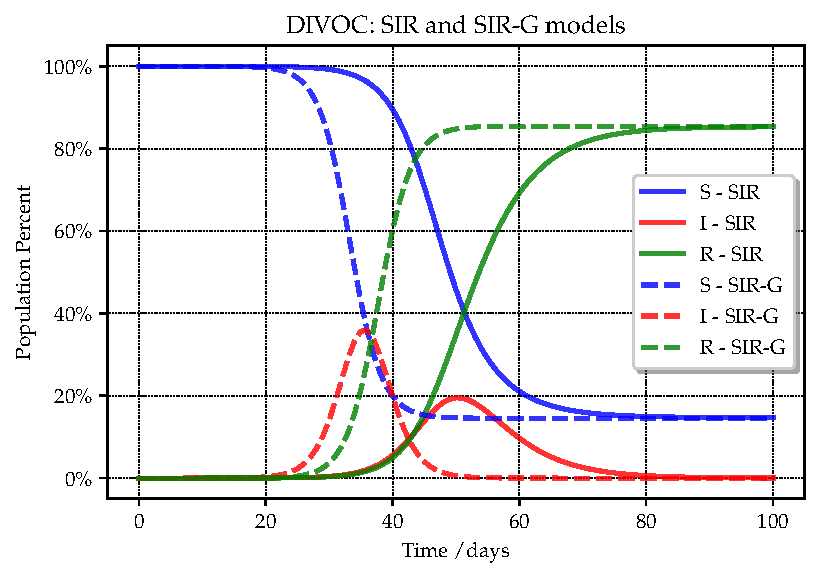
\includegraphics[width=.8\linewidth]{DIVOC-SIR-comp.pdf}
		\caption{$S$, $I$, and $R$ as function of time}
	\end{subfigure}	
	\begin{subfigure}{.45\textwidth}
		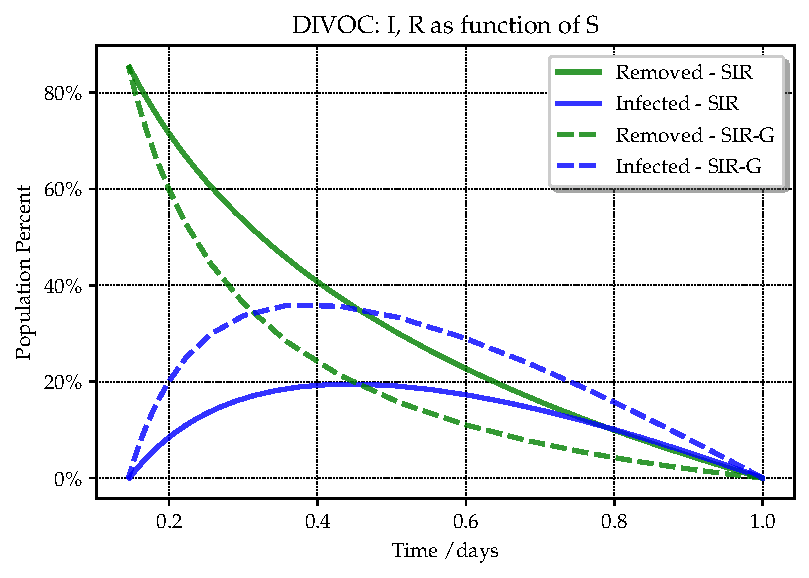
\includegraphics[width=.8\linewidth]{DIVOC-IR-comp.pdf}
		\caption{$R$ and $I$ as function of $S$}
	\end{subfigure}	
	\caption{Comparison of classical SIR with SIR-G}
	\label{fig:comp}
\end{figure}


\subsection{Impact of Variability in SIR-G}

In this section we will use diverse Gamma and Lognormal distributions with various values for the coefficient of variability.

\begin{figure}
	\centering
	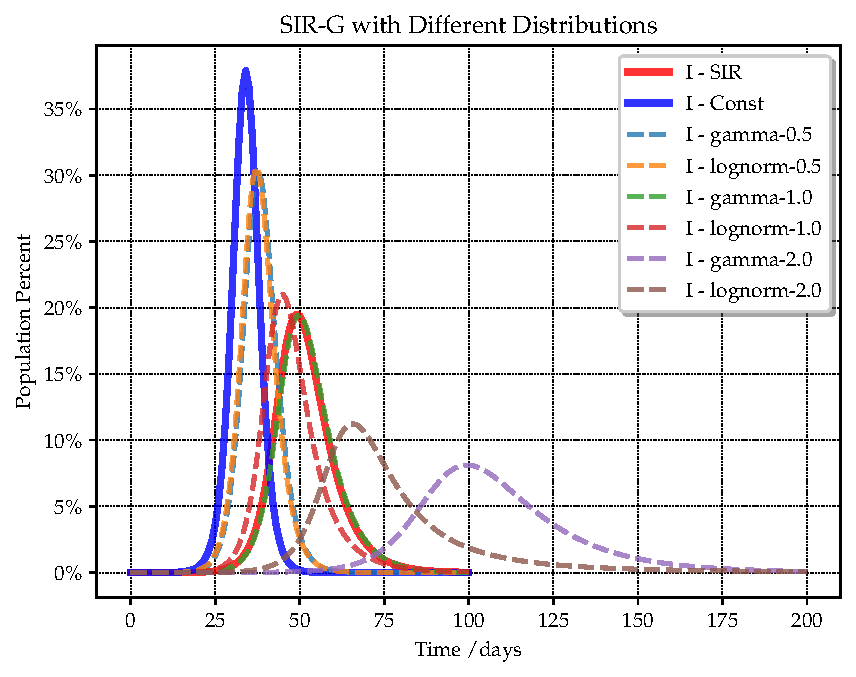
\includegraphics[width=.8\linewidth]{Variance-Analysis.pdf}
	\caption{SIR-G for different variability levels}
	\label{fig:var}
\end{figure}

\section{Epidemic Model with Phase-Type Distributions}\label{sc:PH}


\section{A Multi-stage Epidemic Model}\label{sc:multi}




%% <== End of hints
%%%%%%%%%%%%%%%%%%%%%%%%%%%%%%%%%%%%%%%%%%%%%%%%%%%%%%%%%%%%%



%%%%%%%%%%%%%%%%%%%%%%%%%%%%%%%%%%%%%%%%%%%%%%%%%%%%%%%%%%%%%
%% BIBLIOGRAPHY AND OTHER LISTS
%%%%%%%%%%%%%%%%%%%%%%%%%%%%%%%%%%%%%%%%%%%%%%%%%%%%%%%%%%%%%
%% A small distance to the other stuff in the table of contents (toc)
\addtocontents{toc}{\protect\vspace*{\baselineskip}}

%% The Bibliography
%% ==> You need a file 'literature.bib' for this.
%% ==> You need to run BibTeX for this (Project | Properties... | Uses BibTeX)

% \addcontentsline{toc}{chapter}{Bibliography} %'Bibliography' into toc
%\nocite{*} %Even non-cited BibTeX-Entries will be shown.
% \bibliographystyle{plainnat} %Style of Bibliography: plain / apalike / amsalpha / ...
\bibliographystyle{plain}
\bibliography{Stochastics,Riano,Epidemiology,Manufacturing} %You need a file 'literature.bib' for this.



%%%%%%%%%%%%%%%%%%%%%%%%%%%%%%%%%%%%%%%%%%%%%%%%%%%%%%%%%%%%%
%% APPENDICES
%%%%%%%%%%%%%%%%%%%%%%%%%%%%%%%%%%%%%%%%%%%%%%%%%%%%%%%%%%%%%
\appendix

\section{Appendix: Computing Expected Values of Piece-wise Linear Functions} \label{app:piecewise}
It is convenient to write the function  $\Ab(t)$ in terms of the so-called first order loss function $L(t)=\E{(T-t)^+}$ as follows
\[ \Ab(t) = \gamma \int_t^\infty \Gb(s)ds = \gamma L(t).\]
The advantage of this representation is that the loss function is known for many distributions, and can be efficiently computed without performing actual integration. See, \eg, \cite[Page 14]{burn.ea.10} and \cite[Appendix C]{zipk00}.

\end{document}

